\documentclass[12pt]{article}
\usepackage{amsmath, amssymb}
\usepackage[margin=0.5cm]{geometry}
\usepackage{array}
\usepackage{helvet}
\usepackage{longtable}
\usepackage{tikz-cd}
\usepackage{tikz}
% Add libraries for positioning and arrows
\usetikzlibrary{trees, positioning, arrows}
\usepackage{changepage} % For margin adjustments

\begin{document}

\begin{center}
		{\LARGE\bfseries Special Matrices and their Properties}\par
		\vspace{1em}
\end{center}

% Matrix Type Hierarchy Tree
\begin{center}
  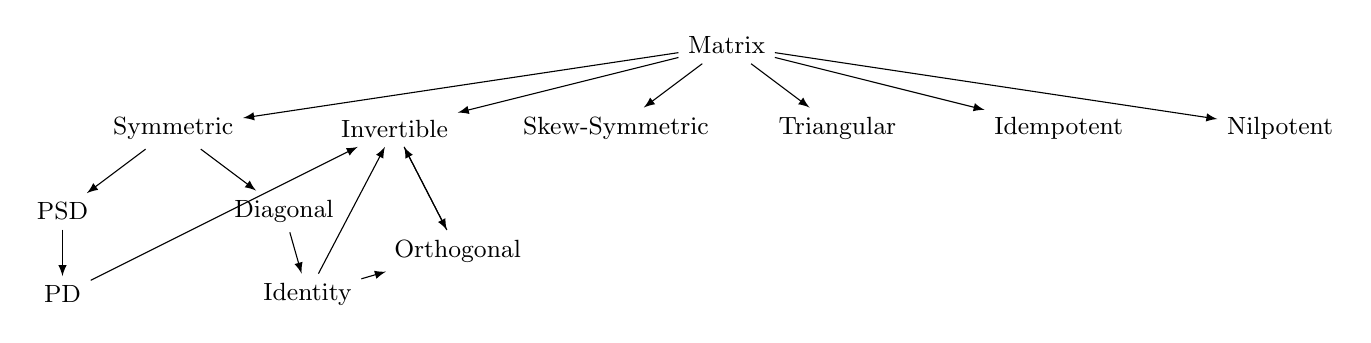
\begin{tikzpicture}[
						level distance=3em, % Adjusted level distance
						every node/.style={font=\small},
						sibling distance=8em, % Adjusted sibling distance
						edge from parent/.style={draw,-latex}
				]
    \node (Matrix) {Matrix}
				child { node (Symmetric) {Symmetric}
						child { node (PSD) {PSD}
								child { node (PD) {PD} }
						}
						child { node (Diagonal) {Diagonal}
								child { node [xshift=0.3cm](Identity) {Identity} }
						}
				}
				child { node (Invertible) {Invertible}[sibling distance=20em]
						child { node [xshift=0.8cm, yshift=-0.5cm](Orthogonal) {Orthogonal} }
				}
				child { node {Skew-Symmetric} }
				child { node {Triangular} }
				child { node {Idempotent} }
				child { node {Nilpotent} };

    % Add arrows for overlaps
    \draw[-latex] (PD) -- (Invertible);
    \draw[-latex] (Identity) -- (Invertible);
    \draw[-latex] (Identity) -- (Orthogonal);
    \draw[-latex] (Orthogonal) -- (Invertible);

  \end{tikzpicture}
  \vspace{0.5em}
  \small{Arrows indicate subset or special case relationships. Additional arrows show overlaps.}
\end{center}

\begin{longtable}{|>{\bfseries}m{3.5cm}|m{5cm}|m{10.5cm}|}
		\hline
		\textbf{Term} & \textbf{Definition} & \textbf{Unique Attributes /
		Key Properties} \\
		\hline
		Diagonal & $a_{ij} = 0$ for $i \ne j$ &
		- Determinant is product of diagonal entries \newline
		- Eigenvalues are diagonal entries \newline
		- $A^k$ is diagonal with entries raised to $k$ \\
		\hline
		Symmetric & $A = A^T$, i.e., $a_{ij} = a_{ji}$ &
		- All eigenvalues are real \newline
		- Eigenvectors for distinct eigenvalues are orthogonal \newline
		- Diagonalizable via orthogonal matrices \\
		\hline
		Identity ($I$) & $I_{ij} = \delta_{ij}$ &
		- $AI = IA = A$ \newline
		- $I^{-1} = I$ \newline
		- All eigenvalues are 1 \\
		\hline
		Invertible (Non-singular) & Exists $A^{-1}$ such that $AA^{-1} =
		A^{-1}A = I$ &
		- $\det(A) \ne 0$ \newline
		- Linearly independent rows and columns \newline
		- No zero eigenvalues \\
		\hline
		Singular & A square matrix with $\det(A) = 0$ &
		- Not invertible \newline
		- May have linearly dependent rows or columns \newline
		- At least one zero eigenvalue \\
		\hline
		Orthogonal & $A^{-1} = A^T$, so $A^T A = I$ &
		- Rows and columns form an orthonormal set \newline
		- Preserves lengths and angles \newline
		- $\det(A) = \pm 1$ \\

		\hline
		Pseudoinverse (Moore--Penrose) & Generalized inverse $A^\dagger$
		satisfying the four Penrose conditions &
		- Always exists and is unique for any matrix \newline
		- If $A \in \mathbb{R}^{m \times n}$ has full column rank ($m \ge
		n$): \newline
		\quad $A^\dagger = (A^T A)^{-1} A^T$, and $A^\dagger A = I_n$ \newline
		- If $A$ has full row rank ($n \ge m$): \newline
		\quad $A^\dagger = A^T (A A^T)^{-1}$, and $A A^\dagger = I_m$ \newline
		- If $A$ is square and invertible: $A^\dagger = A^{-1}$ \newline
		- Used in least-squares solutions and underdetermined systems \\

		\hline
		Positive Definite & $\vec{x}^T A \vec{x} > 0$ for all non-zero $\vec{x}$ &
		- All eigenvalues are positive \newline
		- $\det(A) > 0$ \newline
		- Invertible \\
		\hline
		Positive Semi-Definite & $A = A^T$, $\vec{x}^T A \vec{x} \ge 0$ for all $\vec{x}$ &
		- All eigenvalues are non-negative \newline
		- $\det(A) \ge 0$ \newline
		- Always symmetric \newline
		- Can always be written as $X^T X$ for some $X$ (Gram matrix) \newline
		- Defines a semi-inner product \\
		\hline
		Triangular (Upper / Lower) &
		Upper: $a_{ij} = 0$ for $i > j$; Lower: $a_{ij} = 0$ for $i < j$ &
		- Determinant is product of diagonal entries \newline
		- Eigenvalues are diagonal entries \newline
		- Solves systems efficiently via substitution \\
		\hline
		Skew-Symmetric & $A = -A^T$, so $a_{ii} = 0$ &
		- Eigenvalues are 0 or purely imaginary \newline
		- $\vec{x}^T A \vec{x} = 0$ for all $\vec{x}$ \\
		\hline
		Idempotent & $A^2 = A$ &
		- Used in projection operations \newline
		- Eigenvalues are 0 or 1 \\
		\hline
		Nilpotent & $A^k = 0$ for some $k \in \mathbb{N}$ &
		- All eigenvalues are 0 \\
		\hline
		Orthogonal Projection & Linear transformation $P$ where $P^2 = P$
		and $P = P^T$ &
		- Projects onto a subspace along its orthogonal complement \newline
		- Minimizes distance to the subspace (best approximation) \newline
		- $\text{Im}(P)$ is a subspace; $\text{Ker}(P) = \text{Im}(I - P)$ \\
		\hline
		Linear Map (Transformation) & Function $T: V \rightarrow W$
		satisfying $T(a\vec{x} + b\vec{y}) = aT(\vec{x}) + bT(\vec{y})$ &
		- Represented by a matrix in finite dimensions \newline
		- Preserves linear structure \newline
		- Kernel and image define fundamental subspaces \\
		\hline
		Fundamental Subspaces & Column space, row space, null space, left null space &
		- Column space: span of columns (range of $A$) \newline
		- Row space: span of rows = col space of $A^T$ \newline
		- Null space: solutions to $A\vec{x} = 0$ \newline
		- Left null space: null space of $A^T$ \\
		\hline
		Unitary & $U^\dagger = U^{-1}$, where $U^\dagger$ is the conjugate
		transpose of $U$ &
		- $U^\dagger U = U U^\dagger = I$ \newline
		- Preserves inner products: $\langle U\vec{x}, U\vec{y} \rangle =
		\langle \vec{x}, \vec{y} \rangle$ \newline
		- All eigenvalues lie on the unit circle: $|\lambda| = 1$ \newline
		- Generalization of orthogonal matrices to complex space \\
		\hline

\end{longtable}

\end{document}
